\documentclass[12pt, a4paper]{article}

\usepackage[utf8]{inputenc}
\usepackage[russian]{babel}
\parindent 0pt
\parskip 8pt
\usepackage{amsmath}
\usepackage{amssymb}
\usepackage{array}
\usepackage[left=2.3cm, right=2.3cm, top=2.7cm, bottom=2.7cm, bindingoffset=0cm]{geometry} % headheight=0pt,
\usepackage{hyperref}
\usepackage{graphicx}
\usepackage{multicol}
\usepackage{fancyhdr} 
\usepackage{extramarks}
\usepackage[usenames,dvipsnames]{color}
\usepackage{titlesec}
\usepackage{tikz}
\definecolor{grey}{RGB}{128,128,128}

\pagestyle{fancy}
\fancyhf{}
\lhead{Билет № 1.2}
\chead{Оперативная память: характеристики, типы динамической памяти.}
\rhead{\thepage}
\lfoot{made with Ы}
\cfoot{}
\rfoot{\today}
\renewcommand\headrulewidth{0.4pt}
\renewcommand\footrulewidth{0.4pt}

\titlespacing*{\section}{0pt}{5pt}{0pt}
\titlespacing*{\subsection}{0pt}{5pt}{0pt}
\titlespacing*{\subsubsection}{0pt}{5pt}{0pt}

\begin{document}
\section{Игрушечный модуль памяти}
\begin{figure}[h]
    \centering
    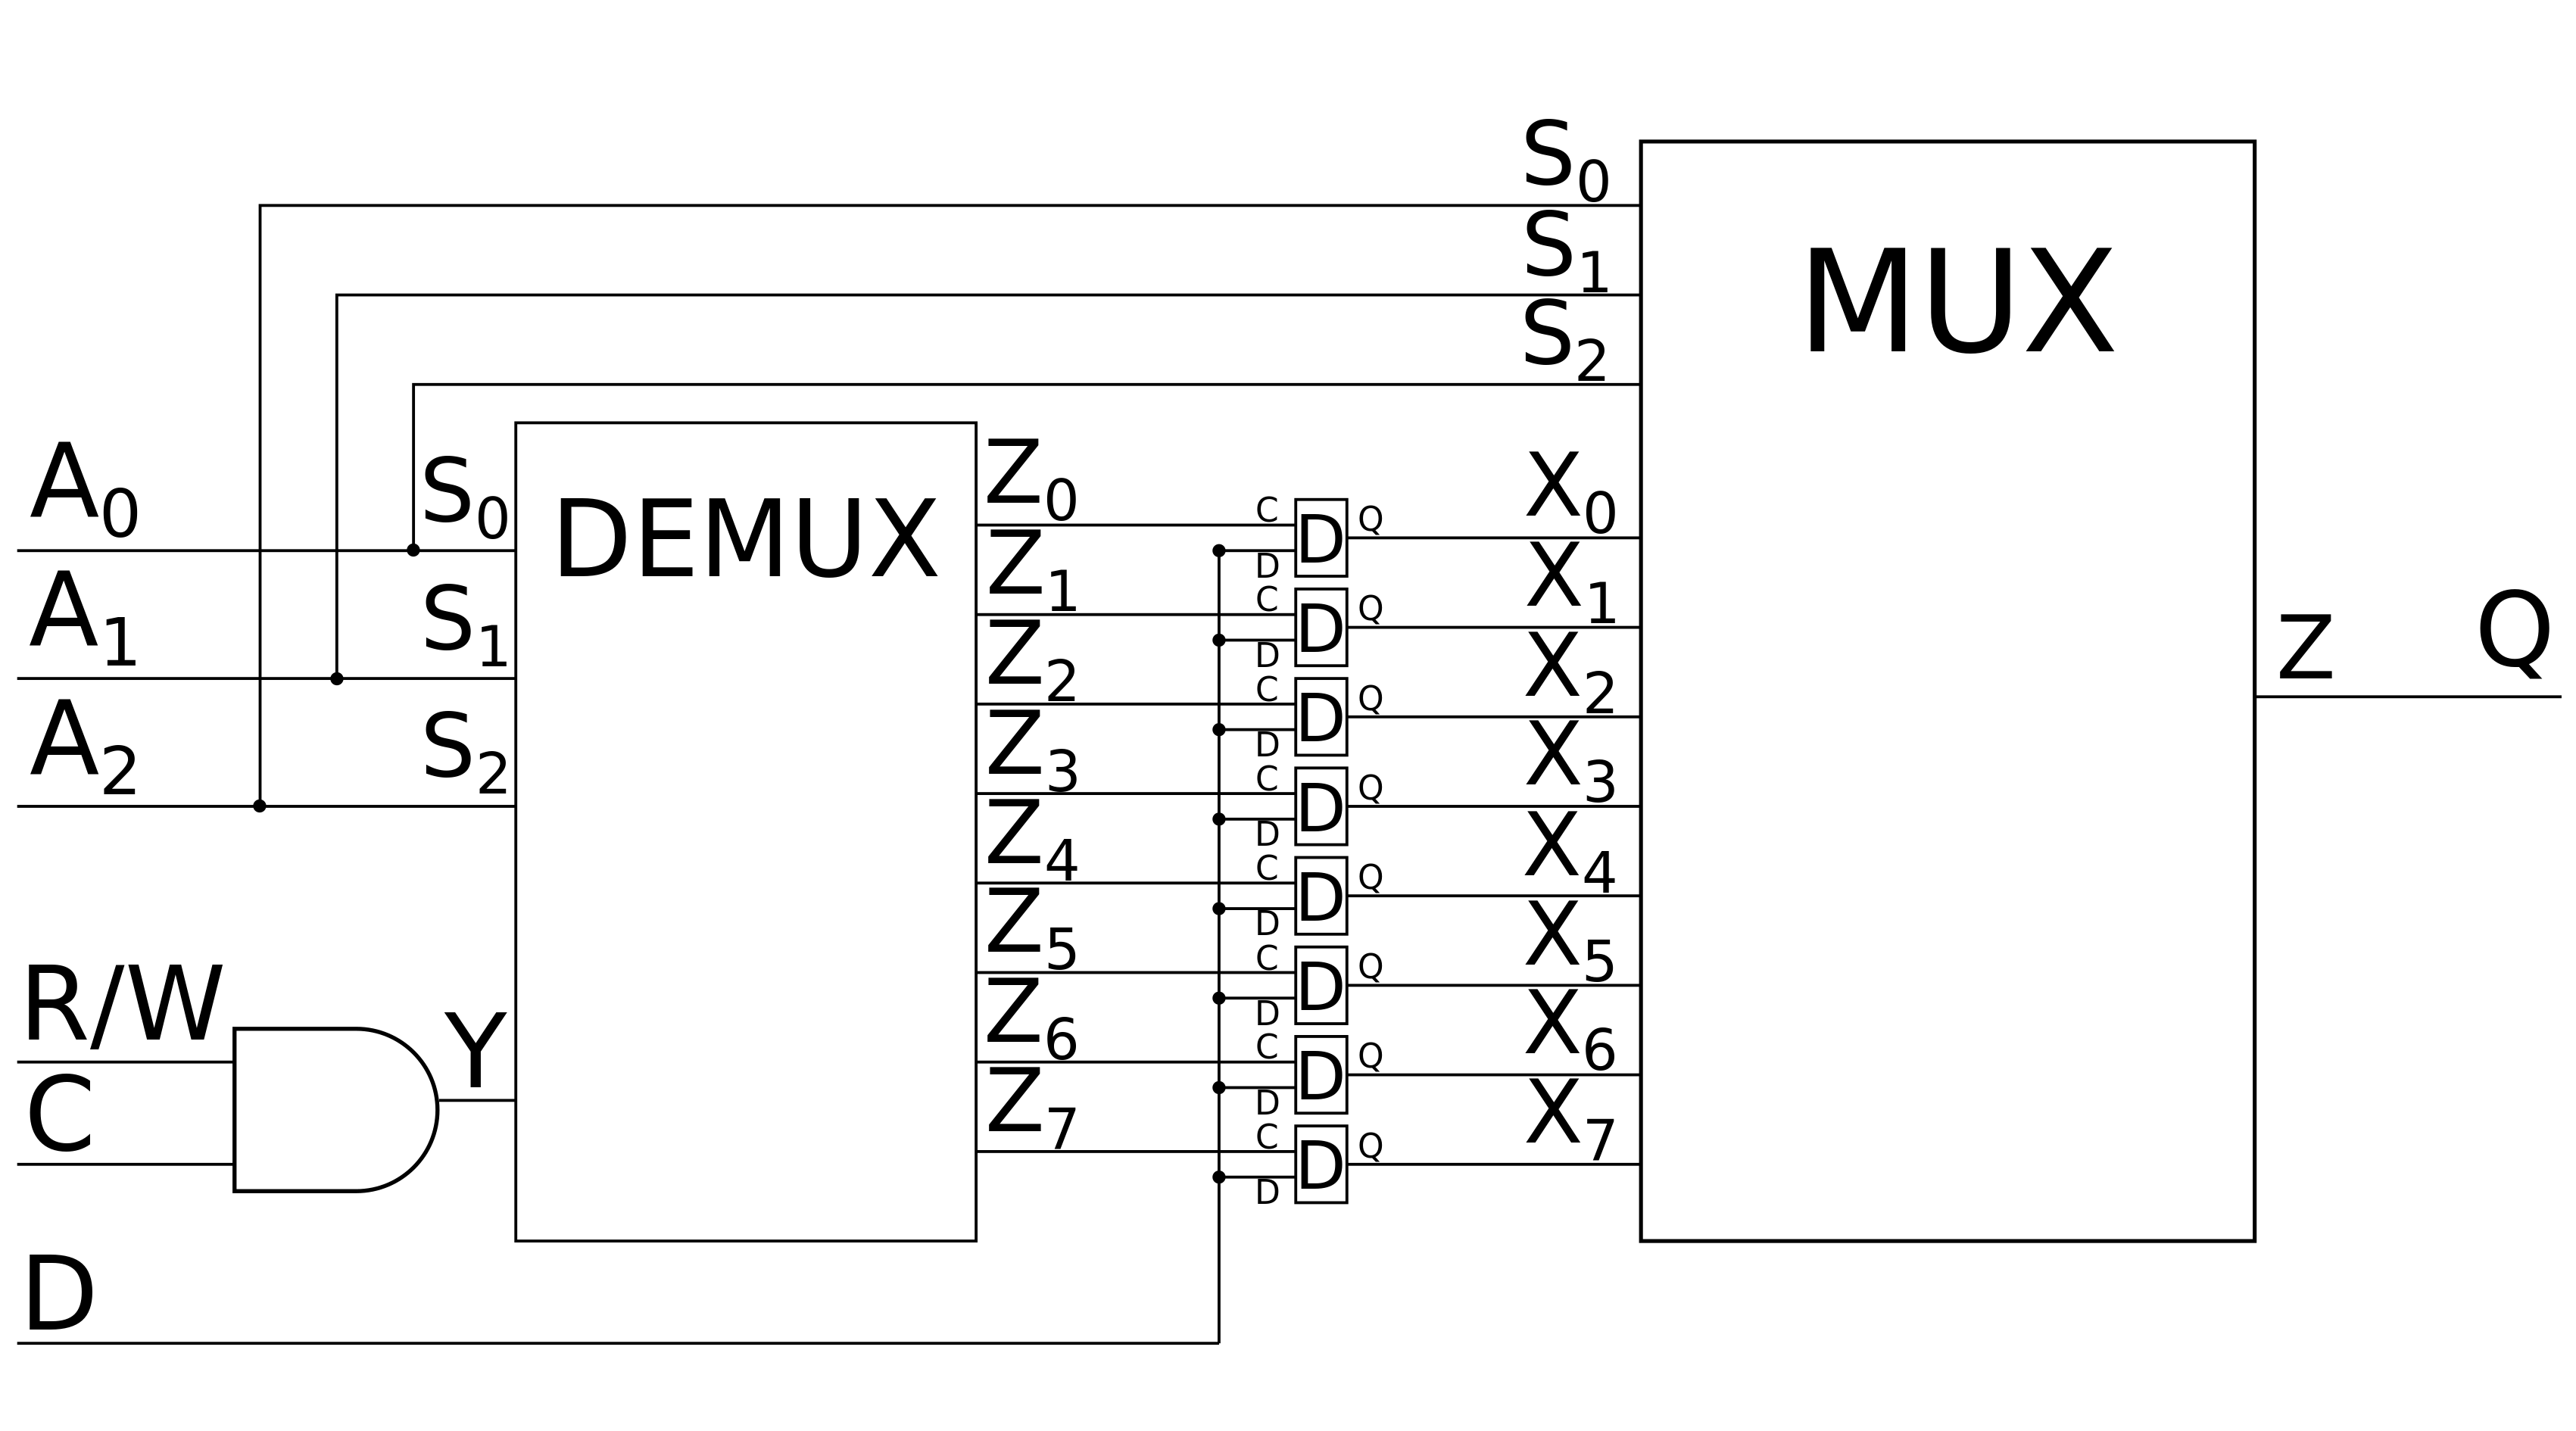
\includegraphics[scale=0.1]{./images/8bitmemory.png}
    \caption{Модуль памяти из D триггеров}
    \label{fig:my_label}
\end{figure}
Это конечно здорово, но никто так не делает. Потому что есть проблемы с масштабируемостью: на один гигабит понадобится слишком много проводов, кроме того будут проблемы с синхронизацией кучи триггеров.
\section{Шина}
\textbf{Шина} - набор проводов и протокол, по которому она используется.\\
\textbf{PCI-E} - внутренняя шина, внешний аналог - Thunderbolt.
\section{Реальный модуль памяти}
\begin{figure}[h]
    \centering
    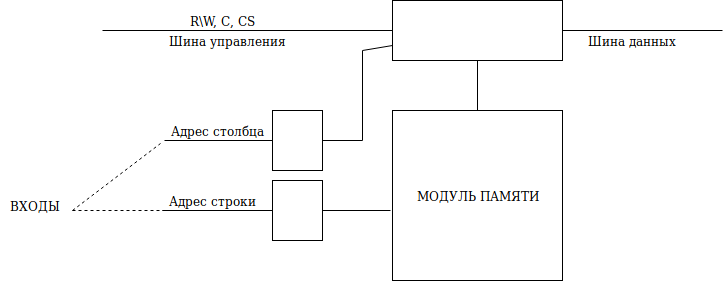
\includegraphics[scale=0.5]{./images/MEM.png}
    \caption{Модуль памяти + контроллер}
    \label{fig:MEM}
\end{figure}
Заметим, что можем сократить число проводов вдвое, т.к. входы $D$ и выходы $Q$ никогда не используются одновременно. Сигнал $R\backslash W$ определяет, как мы используем провода. У нас есть провода и какой-никакой протокол обращения с ними, теперь это шина памяти.\\
У шины памяти есть две "подшины":
\begin{itemize}
    \item Шина адреса. (Строго от контроллера к модулю)
    \item Шина данных. (От контроллера к модулю при записи, наоборот при чтении)
\end{itemize}
Идейно реальный модуль памяти организован в виде двумерной матрицы. Шина адреса тоже можем уменьшить вдвое: на первом такте будем передавать адрес строки, на втором - адрес столбца.
\section{Ячейка памяти}
\subsection{Статическая}
\begin{figure}[h]
    \centering
    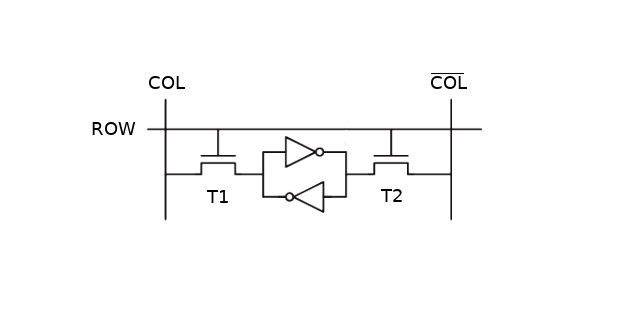
\includegraphics[scale=0.5]{./images/SRAM.png}
    \caption{Шеститранзисторная ячейка статической памяти}
    \label{fig:SRAM}
\end{figure}
Является энергозависимой (т.е. без питания данные теряются).\\
Содержит 5 проводов: $ROW$, $COL$ и $\overline{COL}$, а так же питание и земля.
\subsubsection{Чтение}
В теории, нужно только подать напряжение на $ROW$ и считать значения с $COL$ и $\overline{COL}$.\\
На практике*, $COL$ и $\overline{COL}$ - достаточно длинные провода, и между ними может образоваться ненужное нам электрическое поле. Поэтому, чтобы ускорить чтение, используется более хитрый процесс: сначала на $COL$ и $\overline{COL}$ подается высокое напряжение (логическая \textbf{1}). Затем напряжение подается на $ROW$, транзисторы $T1$ и $T2$ открываются, из-за чего напряжение на одной из линий $COL$ и $\overline{COL}$ чуть-чуть падает. Определяя, на каком проводе напряжение выше, узнаем, что хранилось в ячейке: \textbf{0} или \textbf{1}.
\subsubsection{Запись}
Подаем на $COL$ и $\overline{COL}$ то, что хотим записать. Затем подается напряжение на $ROW$.
\subsubsection{Преимущесва}
\begin{itemize}
    \item Не требует постоянной перезарядки(поэтому и называется статической)
    \item Транзисторы переключаются быстрее, чем заряжается/разряжается конденсатор, поэтому работает быстрее DRAM.
\end{itemize}
\subsubsection{Недостатки}
\begin{itemize}
    \item Дорого
    \item Занимает много места (целых 4/6/8/10 транзисторов на ячейку!)
\end{itemize}
\subsubsection{В итоге}
Используется там, где нужно мало быстрой памяти. Т.е. в кэшах, регистрах.
\subsection{Динамическая}
\begin{figure}
    \centering
    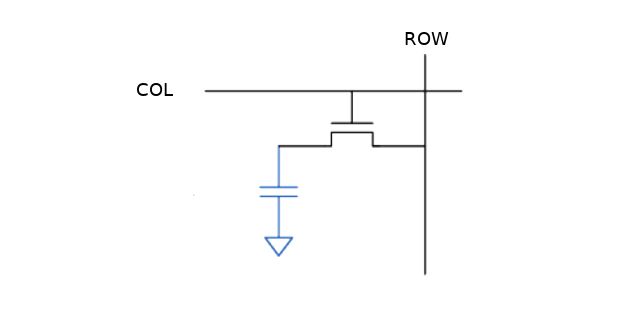
\includegraphics[scale=0.5]{./images/DRAM.png}
    \caption{Ячейка динамической памяти}
    \label{fig:DRAM}
\end{figure}
Тоже является энергозависимой.\\ 
Содержит всего три провода: $COL$, $ROW$ и земля.\\
Состоит из одного транзистора и одного конденсатора.
\subsubsection{Чтение}
Читаем сразу всю строку. В теории: подаем напряжение на $ROW$ и замеряем значения. Не забываем перезарядить, т.к. у конденсаторов есть свойство разряжаться при чтении.\\
На практике*: подаём половинку напряжения логической \textbf{1} на столбцы. Затем подаем напряжение на $ROW$. Замеряем изменения: если стало меньше, чем подали - там \textbf{0}, стало больше - \textbf{1}.
\subsubsection{Запись}
Очень просто: подаем напряжение на $ROW$, затем подаем нужное напряжение на $COL$.
\subsection{Преимущества}
\begin{itemize}
    \item Дешево
    \item Каждая ячейка занимает мало места -> можно сделать больше ячеек.
\end{itemize}
\subsubsection{Недостатки}
\begin{itemize}
    \item После чтения нужно перезаряжать конденсаторы.
    \item Конденсаторы очень маленькие, имеют очень маленькую ёмкость, поэтому они разряжаются сами по себе за очень быстро. Нужно постоянно перезаряжать (считывать строку и записывать обратно).\\
    Этим может заниматься программист или контроллер памяти. В наше время этим занимается контроллер памяти.
    \item Все эти фокусы с конденсаторами достаточно долгие.
\end{itemize}
\subsubsection{В итоге}
Используется там где нужно много дешевой памяти. RAM, например.
\section{Лирическое отступление}
\subsection{DMA и PIO}
\textbf{DMA} (\textit{Direct Memory Access}) - фича, которая позволяет некоторым аппаратным устройствам обращаться к памяти минуя процессор. Возникла потому что если каждое медленное устройство, которому нужно что-то от памяти, будет дергать быстрый процессор - всем станет очень грустно по скорости. Типичный представитель DMA устройства - HDD.\\
Как работает: CPU инициирует/разрешает передачу данных от одного устройства другому, а потом занимается своими делами, пока не получит прерывание (когда DMA контроллер закончит передачу данных).\\
\textbf{PIO} (\textit{Programmed Input/Output}) - подход, когда процессор во время операции чтения/записи не может ничего делать. Если включить такой режим для HDD (вроде как можно было в BIOS), можно получить хороший такой проигрыш в скорости.
\subsection{SATA}
\textbf{SATA} (\textit{Serial ATA}) - популярный интерфейс для подключения долговременной памяти. Можно подключать и HDD, и SSD, и SSHD.
\subsection{Чипсет}
Процессор очень быстрый, а все остальные не очень. Поэтому давайте высокоскоростные устройства подключим поближе к процессору (северный мост), а медленные - подальше (южный мост).
\begin{figure}[h]
    \centering
    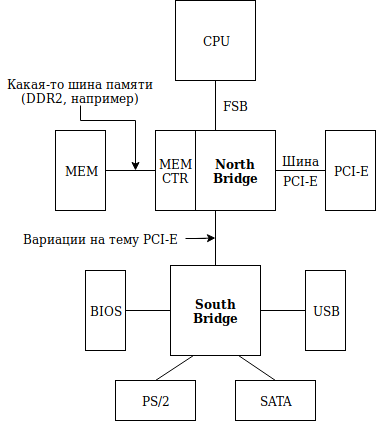
\includegraphics[scale=0.3]{./images/NBSB.png}
    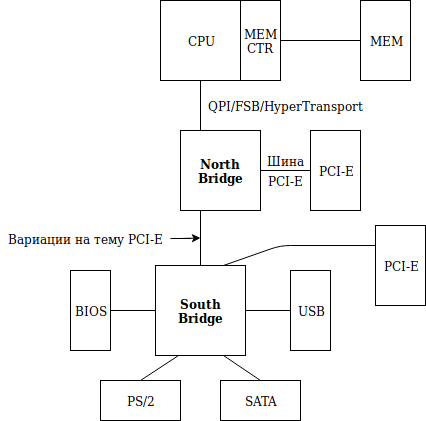
\includegraphics[scale=0.3]{./images/NBSB1.png}
    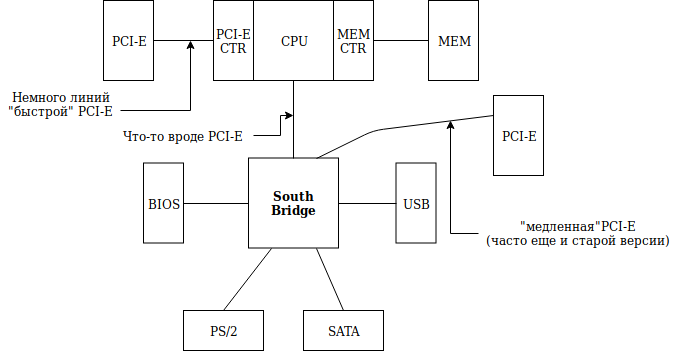
\includegraphics[scale=0.3]{./images/NBSB2.png}
    \caption{Вариации чипсета. Вправо новее}
    \label{fig:CHIPSET0}
\end{figure}
Можно заметить, что в современности наблюдается тенденция засунуть весь северный мост на один кристалл к процессору, чтобы быстрее. Принцип SoC - "система на кристалле".
\begin{figure}[h]
    \centering
    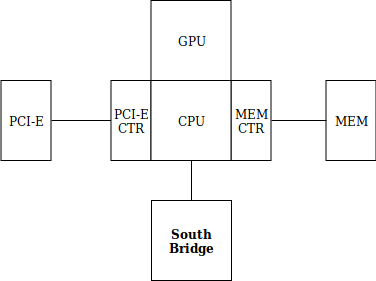
\includegraphics[scale=0.4]{./images/SOC.png}
    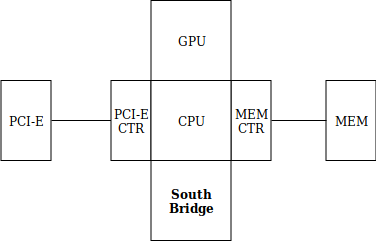
\includegraphics[scale=0.4]{./images/Mobile.png}
    \caption{Слева еще более новая вариация. Справа мобильный чипсет}
    \label{fig:CHIPSET1}
\end{figure}
\subsection{Поток сознания. Что-то из этого полезно, но это не точно}
\begin{itemize}
\item \textbf{PS$\backslash$2 не хотспот, а еще для него не нужен драйвер, в отличие от USB}
\item Во времена DOS внутри каждой програмки (например игрушки) была программа конфигурации. Сначала нужно было запустить её, потом саму программу. Если программа не умела в имеющееся железо - ОЖВП.
\item Одна из задач операционной системы - построение абстракции для работы на любом железе. Следовательно можно использовать API, а ОС будет передавать управление драйверу. Драйвер транслирует команды API в команды для железки.\\
Драйверы системно-зависимые.
\item Вставьте сюда вашу любимую байку про заговор NVIDIA.
\end{itemize}
\section{Источники информации}
\begin{itemize}
    \item Википедия
    \item Конспекты @ntwwwnt (есть в гуглопапке)
\end{itemize}
\end{document}